\documentclass{standalone}

\usepackage{amsmath}
\usepackage{amssymb}
\usepackage{tikz}
\usetikzlibrary{matrix,positioning,decorations.pathreplacing}

\newcommand{\code}[1]{\texttt{#1}}
\newcommand{\X}{\mathbb{X}}

\begin{document}
\pagestyle{empty}
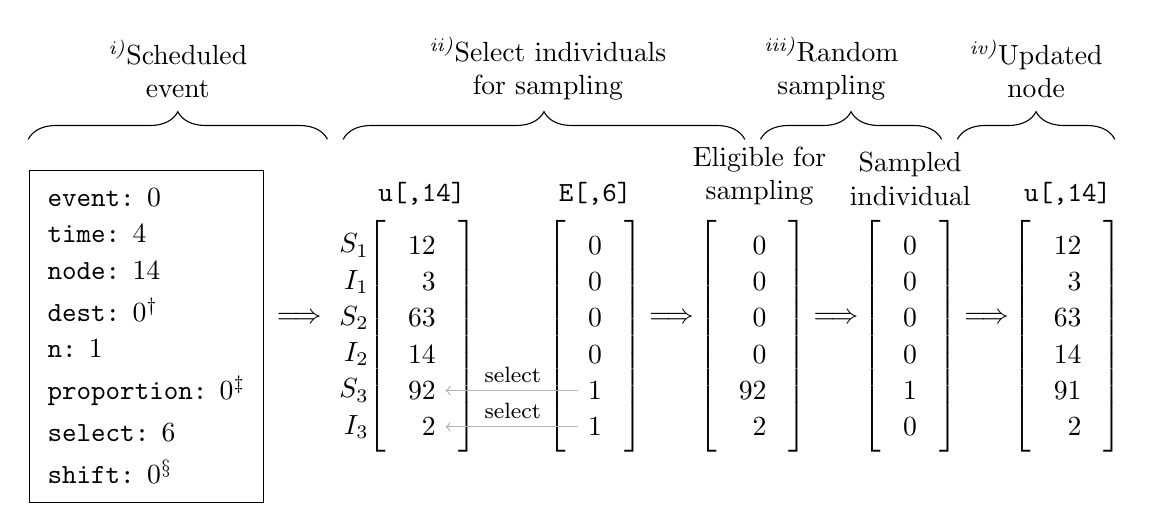
\begin{tikzpicture}[node distance=1ex]

  \draw [decorate,decoration={brace,amplitude=10pt},rotate=-90]
  (-2.5,-4.0) -- (-2.5,-0.2);

  \node [align=center] at (-2.1,3.4) {$^\textit{i)}$Scheduled
    \\ event};

  \matrix [matrix of nodes,
           draw,
           column 1/.style={anchor=base west}] at (-2.5,0)
          {
            \code{event:} 0 \\
            \code{time:} 4 \\
            \code{node:} 14 \\
            \code{dest:} 0$^\dag$ \\
            \code{n:} 1 \\
            \code{proportion:} 0$^\ddag$ \\
            \code{select:} 6 \\
            \code{shift:} 0$^\S$ \\
          };

  \draw [decorate,decoration={brace,amplitude=10pt},rotate=-90]
  (-2.5,0) -- (-2.5,5.1);

  \node [align=center] at (2.6,3.4) {$^\textit{ii)}$Select individuals
    \\ for sampling};

  \draw [decorate,decoration={brace,amplitude=10pt},rotate=-90]
  (-2.5,5.3) -- (-2.5,7.6);

  \node [align=center] at (6.2,3.4) {$^\textit{iii)}$Random
    \\ sampling};

  \draw [decorate,decoration={brace,amplitude=10pt},rotate=-90]
  (-2.5,7.8) -- (-2.5,9.8);

  \node [align=center] at (8.8,3.4) {$^\textit{iv)}$Updated \\ node};

  \matrix (u) [matrix of math nodes,
               left delimiter={[},
               right delimiter={]},
               column 1/.style={anchor=base east}] at (1,0)
          {
            12 \\
             3 \\
            63 \\
            14 \\
            92 \\
             2 \\
          };

          \node [above=of u-1-1.north] {\code{u[,14]}};
          \node [left=of u-3-1.east,xshift=-1.3cm] {$\Longrightarrow$};
          \node [left=of u-1-1.east,xshift=-0.7cm] {$S_1$};
          \node [left=of u-2-1.east,xshift=-0.7cm] {$I_1$};
          \node [left=of u-3-1.east,xshift=-0.7cm] {$S_2$};
          \node [left=of u-4-1.east,xshift=-0.7cm] {$I_2$};
          \node [left=of u-5-1.east,xshift=-0.7cm] {$S_3$};
          \node [left=of u-6-1.east,xshift=-0.7cm] {$I_3$};

  \matrix (E) [matrix of math nodes,
               left delimiter={[},
               right delimiter={]},
               column 1/.style={anchor=base east}] at (3.2,0)
          {
            0 \\
            0 \\
            0 \\
            0 \\
            1 \\
            1 \\
          };
          \node [above=of E-1-1.north] {\code{E[,6]}};
          \node [right=of E-3-1.east,xshift=0.2cm] {$\Longrightarrow$};

          \draw[->,black!30] (E-5-1.west) -- (u-5-1.east);
          \node [left=of E-5-1.west,xshift=-0.2cm,yshift=0.2cm]
                {\footnotesize{select}};

          \draw[->,black!30] (E-6-1.west) -- (u-6-1.east);
          \node [left=of E-6-1.west,xshift=-0.2cm,yshift=0.2cm]
                {\footnotesize{select}};

  \matrix (Selected) [matrix of math nodes,
                      left delimiter={[},
                      right delimiter={]},
                      column 1/.style={anchor=base east}] at (5.2,0)
          {
             0 \\
             0 \\
             0 \\
             0 \\
            92 \\
             2 \\
          };

          \node [above=of Selected-1-1.north, align=center] {Eligible
            for \\ sampling};
          \node [right=of Selected-3-1.east,xshift=0.2cm] {$\Longrightarrow$};

  \matrix (Sampled) [matrix of math nodes,
                      left delimiter={[},
                      right delimiter={]},
                      column 1/.style={anchor=base east}] at (7.2,0)
          {
             0 \\
             0 \\
             0 \\
             0 \\
             1 \\
             0 \\
          };

          \node [above=of Sampled-1-1.north, align=center] {Sampled
            \\ individual};
          \node [right=of Sampled-3-1.east,xshift=0.2cm] {$\Longrightarrow$};

  \matrix (uNew) [matrix of math nodes,
                  left delimiter={[},
                  right delimiter={]},
                  column 1/.style={anchor=base east}] at (9.2,0)
          {
            12 \\
             3 \\
            63 \\
            14 \\
            91 \\
             2 \\
          };

          \node [above=of uNew-1-1.north] {\code{u[,14]}};

\end{tikzpicture}

\end{document}
